%pdflatex -halt-on-error -aux-directory=tmp -output-directory=tmp rapport.tex%

\documentclass{article}
\usepackage{amsmath}
\usepackage[utf8]{inputenc}
\usepackage[T1]{fontenc}
\usepackage{graphicx}
\usepackage{hyperref}
\usepackage{listings}
\lstset{
  literate=
  {á}{{\'a}}1 {é}{{\'e}}1 {í}{{\'i}}1 {ó}{{\'o}}1 {ú}{{\'u}}1
  {Á}{{\'A}}1 {É}{{\'E}}1 {Í}{{\'I}}1 {Ó}{{\'O}}1 {Ú}{{\'U}}1
  {à}{{\`a}}1 {è}{{\`e}}1 {ì}{{\`i}}1 {ò}{{\`o}}1 {ù}{{\`u}}1
  {À}{{\`A}}1 {È}{{\'E}}1 {Ì}{{\`I}}1 {Ò}{{\`O}}1 {Ù}{{\`U}}1
  {ä}{{\"a}}1 {ë}{{\"e}}1 {ï}{{\"i}}1 {ö}{{\"o}}1 {ü}{{\"u}}1
  {Ä}{{\"A}}1 {Ë}{{\"E}}1 {Ï}{{\"I}}1 {Ö}{{\"O}}1 {Ü}{{\"U}}1
  {â}{{\^a}}1 {ê}{{\^e}}1 {î}{{\^i}}1 {ô}{{\^o}}1 {û}{{\^u}}1
  {Â}{{\^A}}1 {Ê}{{\^E}}1 {Î}{{\^I}}1 {Ô}{{\^O}}1 {Û}{{\^U}}1
  {œ}{{\oe}}1 {Œ}{{\OE}}1 {æ}{{\ae}}1 {Æ}{{\AE}}1 {ß}{{\ss}}1
  {ű}{{\H{u}}}1 {Ű}{{\H{U}}}1 {ő}{{\H{o}}}1 {Ő}{{\H{O}}}1
  {ç}{{\c c}}1 {Ç}{{\c C}}1 {ø}{{\o}}1 {å}{{\r a}}1 {Å}{{\r A}}1
  {€}{{\EUR}}1 {£}{{\pounds}}1
}

\def\changemargin#1#2{\list{}{\rightmargin#2\leftmargin#1}\item[]}
\let\endchangemargin=\endlist 

\title{Rapport de projet : Jeu de Dames en réseau}
\author{Anthony Bertrand, Quentin Bandera}
\date{}

\begin{document}
    \pagenumbering{gobble}
    \maketitle
    \tableofcontents
    \newpage
    \pagenumbering{arabic}
    \section{Introduction}
        Lors de nos études en L3 Informatique, nous avons dû implémenter un jeu de Dame en réseau. Le but de ce projet
        est de mettre en pratique les connaissances acquises aussi bien en cours magistral qu'en travaux pratiques.
        Nous allons tout d'abord revenir sur les règles à implémenter pour le jeu de Dame. Nous verrons ensuite quels sont
        les choix à notre disposition en ce qui concerne les protocoles réseaux, ainsi que les structure que nous allons utiliser.
        Enfin, nous regarderons en détail le travail effectué ainsi que les potentielles améliorations.

    \section{Le jeu de Dame}
    \subsection{Origine}
        Le jeu de dame (Draughts ou Checkers en anglais) est un jeu pour deux joueurs se jouant avec un plateau. Les origines du
        jeu viendraient de l'Egypte antique, vers -1500 avant Jésus Christ.

    \subsection{Règles du jeux}
    \subsubsection{But du jeu}
        Le but du jeu de dames est de prendre toutes les pièces de l'adversaire. Pour se faire, les joueurs disposent de 20 pièces
        disposées sur le plateau et séparées d'une case. On joue généralement sur les cases noires (ref Figure 1). La taille du plateau
        peut varier suivant les règles mais la version du jeu la plus connue est celle qui se joue sur un plateau 10x10 cases.
        
        \begin{figure}[!htp]
            \centerline{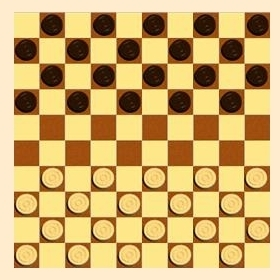
\includegraphics[scale=0.5]{images/dames.jpg}}
            \caption{\label{étiquette} plateau de jeu}
        \end{figure}
        
    \subsubsection{Le déplacement des pièces}
        Lors de son tour d'action, le joueur peut déplacer l'un de ses pions vers une case noire adjacente (il effectue donc un
        déplacement diagonal). Le joueur ne peut pas faire reculer ses pièces, il ne peut se déplacer qu'en avant (sauf pour 
        les prises). Si une pièce est au bord droit ou gauche du plateau, elle n'a donc qu'un seul déplacement disponible. Le joueur
        ne peut pas déplacer sa pièce sur une case déjà occupée par une pièce. (ref Figure 2)

    \subsubsection{Le déplacement des dames}
        Le déplacement d'une dame est beaucoup moins limité. Ces dernières peuvent se déplacer en avant et en arrière. Elle peuvent
        également se déplacer d'autant de cases qu'elle veulent, du moment qu'elle ne rencontre pas d'obstacle (une autre pièce ou
        le bord du plateau). (ref Figure 2)

        \begin{figure}[!htp]
            \centerline{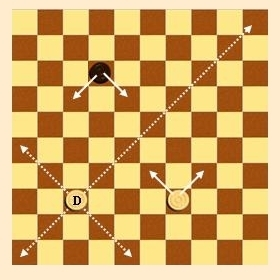
\includegraphics[scale=0.5]{images/deplacement.jpg}}
            \caption{\label{étiquette} déplacements}
        \end{figure}

    \subsubsection{La prise avec des pièces}
        Pour prendre une pièce de l'adversaire, il faut que l'une des pièces du joueur soit adjacente à une pièce de l'adversaire et que
        la case derrière cette dernière soit vide. Le but lors des déplacements de vos pièces sera donc d'éviter à tout prix de laisser
        une pièce sans défenses. La prise en arrière est possible ! (ref Figure 3)

    \subsubsection{La prise avec des dames}
        Comme pour les déplacements, la dame n'a pas besoin d'être adjacente au pion qu'elle veut prendre. Elle peut se déplacer
        d'autant de cases qu'elle veut du moment qu'elle ne rencontre pas d'obstacle entre elle et le pion, et du moment que la case
        derrière le pion est vide. Si les autres cases derrière le pion sont aussi vides, elle peut choisir de s'arreter sur l'une d'elles.
        (ref Figure 4)

    \subsubsection{Les rafles}
        Après avoir prit une pièce de l'adversaire, le joueur peut continuer de prendre d'autre pièces avec le même pion s'il en a la possibilité
        (et il le doit !). La rafle est beaucoup plus simple avec une dame de par ses mouvements moins restreints (ref Figure 3 et 4)

        \begin{figure}[!htp]
            \centerline{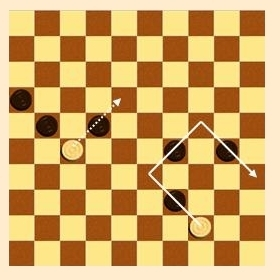
\includegraphics[scale=0.5]{images/prises.jpg}}
            \caption{\label{étiquette} prise simple et rafle}
        \end{figure}

        \begin{figure}[!htp]
            \centerline{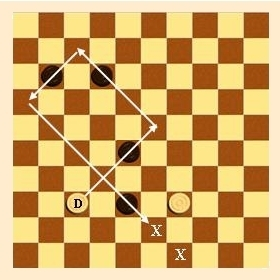
\includegraphics[scale=0.5]{images/prise_dame.jpg}}
            \caption{\label{étiquette} rafle avec une dame}
        \end{figure}

    \subsubsection{Création des dames}
        Lorsqu'une pièce arrive de l'autre coté du plateau, sur la toute dernière rangé, et qu'elle ne peut plus avancer, elle devient une dame.
        Comme vu précédemment, les dames ont une plus grande liberté de déplacement et peuvent se déplacer en arrière. Il est donc dans l'interêt
        du joueur de créer des dames en empêchant la création de dames adverses.

    \section{Etude du problème}
    \subsection{Partie réseau}
    \subsubsection{Choix du protocole de transport}
        Dans le monde du jeu vidéo en ligne, le protocole UDP est très souvent utilisé. UDP possède une faible latence pour le traitement
        ce qui est l'élement recherché dans des jeux nerveux comme Overwatch, League of Legends, Unreal Tournament etc... Dans notre
        cas, le jeu se fera en tour par tour. Notre choix se porte donc sur TCP car nous ne voulons pas de perte de paquet lorsque le joueur
        valide son coup.\\
        Nous aurions pu utiliser un protocole applicatif existant, se basant sur UDP, voire même créer notre propre protocole mais par soucis
        de temps, nous nous contenterons de TCP.

    \subsection{Partie algorithmique du jeu de dames}
    \subsubsection{Structures utilisées}
        Afin de mener à bien ce projet, nous avons décidé de ne pas utiliser de structures trop complexes. Le plateau de jeu est représenté
        par un tableau à une dimension. Nous simulons la deuxième dimension du tableau en utilisant une variable i, j et une constante pour
        le modulo. Une case du plateau avec un tableau à deux dimensions ressemblerai à $plateau[i][j]$. Avec notre implémentation, elle
        ressemble à $plateau[i*CONSTANTE + j]$, la constante étant le nombre de conlonne du plateau.\\
        Nous avons défini une structure $Pion$ avec une coordonée $x$ et une coordonnée $y$ afin de pouvoir transmettre facilement des
        positions sur le plateau au serveur.
        Enfin, nous avons utilisé des constantes définies dans le fichier dame.h afin de faciliter la lecture de code ainsi que les éventuels
        changements.

        \begin{changemargin}{-1cm}{-1cm}
            \lstinputlisting[language=C, firstline=7, lastline=20]{dame.h}
        \end{changemargin}

    \section{Travail effectué}
        Avant de commencé cette partie, nous tenons à préciser que ce projet a dû être réalisé en deux semaine, par des étudiants
        ayant deux mois d'expérience dans le domaine du réseau. Le temps étant la ressource qui nous fit le plus défaut, nous avons
        décidé de nous concentrer au maximum sur la partie réseau et non sur la partie algorithmique du jeu de Dame.
    \subsection{Echanges TCP}
        Comme dit plus haut, nous avons décidé d'utiliser le protocole TCP au niveau de la couche de transport. Nous allons présenter
        dans cette section les algorithmes implémentés pour la gestion du protocole TCP.
    \subsubsection{Le serveur}
        Dans notre serveur, nous utilisons un tableau d'entier $connfd[2]$ afin de stocker les adresses de nos deux clients. Nous créons
        ensuite la socket et la stockons dans $sockfd$.

        \begin{changemargin}{-2cm}{-2cm}
            \lstinputlisting[language=C, firstline=24, lastline=29]{serverTCP.c}
        \end{changemargin}

        Nous configurons ensuite notre structure $sockaddr\_in$ pour le TCP :

        \begin{changemargin}{-2cm}{-2cm}
            \lstinputlisting[language=C, firstline=31, lastline=33]{serverTCP.c}
        \end{changemargin}

        Nous lions ensuite la socket à l'adresse IP :

        \begin{changemargin}{-2cm}{-2cm}
            \lstinputlisting[language=C, firstline=35, lastline=40]{serverTCP.c}
        \end{changemargin}
        
        Nous mettons notre serveur sur écoute afin de pouvoir accepter des clients :

        \begin{changemargin}{-2cm}{-2cm}
            \lstinputlisting[language=C, firstline=42, lastline=48]{serverTCP.c}
        \end{changemargin}

        Puis nous acceptons nos deux clients :

        \begin{changemargin}{-2cm}{-2cm}
            \lstinputlisting[language=C, firstline=53, lastline=63]{serverTCP.c}
        \end{changemargin}

        Ces étapes préliminaires sont indispensables pour que les clients communiquent avec le serveur.
        Après avoir établie la connection entre les clients et le serveur, nous initialisons le plateau de jeu et nous commençons 
        la boucle de jeu

        \begin{changemargin}{-2cm}{-2cm}
            \lstinputlisting[language=C, firstline=67, lastline=79]{serverTCP.c}
        \end{changemargin}

        Dans cette boucle de jeu, le serveur commence par jouer avec le joueur 1. Il lui envoie le plateau de jeu puis lui demande de
        choisir le pion à déplacer. Ensuite, il reçoit les coordonnées envoyées par le joueur 1 avant de passer au joueur 2.\\
        Nous n'avons pas implémenté les déplacements dans le serveur par manque de temps, mais nous affichons les structures
        reçues afin de montrer que les échanges sont opérationnels. De plus, nous ne demandons qu'une seule paire de coordonées
        alors qu'il nous en faudrai une seconde (pour la destination du coup à jouer).


    \subsubsection{Le client}
        Comme pour le serveur, le client doit passer par plusieurs étapes afin d'établir une connection. Il doit dans l'ordre créer 
        la socket, configurer sa structure $sockaddr\_in$ (son adresse) puis se connecter au serveur TCP.

        \begin{changemargin}{-2cm}{-2cm}
            \lstinputlisting[language=C, firstline=12, lastline=39]{clientTCP.c}
        \end{changemargin}

        Ensuite, il entame également sa boucle de jeu où il va recevoir le plateau de jeu ainsi que les instructions du serveur.
        Le joueur doit ensuite saisir les coordonnées du pion à jouer afin que l'algorithme du client les envoie au serveur. Le joueur
        doit ensuite attendre que l'autre joueur ait fini son tour d'action.

        \begin{changemargin}{-2cm}{-2cm}
            \lstinputlisting[language=C, firstline=41, lastline=52]{clientTCP.c}
        \end{changemargin}

    \subsubsection{Les échanges}
        Lors de la partie, le serveur envoie régulièrement le plateau de jeu à ses joueurs, ainsi que les consignes à suivre pour
        ces derniers. Nous envoyons donc un tableau d'entier et des chaines de caractères.\\
        Les clients, eux, envoient une structure $Pion$ constituée de la coordonnée $x$ et $y$ de la pièce qu'ils veulent jouer 
        ou de la case destination.

    \subsection{Le jeu de dames}
    \subsubsection{Initialisation}
        Avant de commencer la partie, il faut créer le plateau de jeu avec les pièces déjà placées. Ceci est fait dans la fonction
        $init\_game()$

        \begin{changemargin}{-2cm}{-2cm}
            \lstinputlisting[language=C, firstline=3, lastline=32]{dame.c}
        \end{changemargin}

    \subsubsection{Jouer un coup}
        Cette partie n'a pas encore été implémentée en réseau mais a été réflechie et codée dans le fichier dame.c\\
        Afin de jouer un coup, il faut tout d'abord choisir la pièce à déplacer. L'algorithme s'assure que le joueur sélectionne
        bien l'une de ses pièces

        \begin{changemargin}{-2cm}{-2cm}
            \lstinputlisting[language=C, firstline=92, lastline=100]{dame.c}
        \end{changemargin}

        Ensuite, le joueur doit choisir la case destination. Comme pour le choix précédent, l'algorithme s'assure que la destination
        est bien une case vide.

        \begin{changemargin}{-2cm}{-2cm}
            \lstinputlisting[language=C, firstline=102, lastline=108]{dame.c}
        \end{changemargin}

        Finalement, une fonction est appelée pour faire d'autres vérifications comme la validité du coup (déplacement diagonal)
        ou dans le cas d'une prise, vérifier qu'il y a bien une pièce de l'adversaire à prendre. Cette fonction permet de changer la
        valeur d'une variable booléenne qui fait boucler l'algorithme jusqu'à ce que le coup soit enfin valide.

    \subsubsection{L'affichage}
        L'affichage est disponible uniquement dans le terminal pour le moment. Nous utilisons des boucles $for$ afin d'afficher le
        contenu de notre tableau $plateau[]$ en séparant chaque éléments par le caractère "|" afin de simuler les cases du plateau.
        Nous avons également rajouté des chiffres sur le coté afin de voir plus facilement à quelle ligne nous sommes. La même chose
        pour les colonnes arrive bientôt.

        \begin{changemargin}{-2cm}{-2cm}
            \lstinputlisting[language=C, firstline=124, lastline=137]{dame.c}
        \end{changemargin}


    \subsubsection{Fin de la partie}
        Afin de savoir si la partie est finie, on a créer une fonction à appeler après chaque coup comportant une prise, qui vérifie
        que le nombre de pions blancs ou noirs n'est pas égal à 0. Si c'est le cas, la fonction retourne $TRUE$ et la partie est fini.
        Le gagnant est la dernière personne à avoir joué.


    \section{Améliorations possibles}
        Il est difficile de faire une partie sur des améliorations possibles quand le plus gros du travail reste à faire,
        mais c'est une partie qui nous tient à coeur car ce projet étant sur un dépot git, il nous sera très facile de le continuer
        sur notre temps libre.\\
        Parmis ces améliorations, il y a celle du plateau de jeu. Etant composé à moitié de case blanches, et l'autre de case noires, et n'utilisant
        que ces dernières, il devrait être possible de réduire la taille stockée en mémoire. C'est une amélioration très légère, mais elle peut
        être très utile car nous envoyons le plateau de jeu assez souvent entre le serveur et les clients. Réduire la taille des paquets envoyés
        reste une priorité en réseau.\\
        D'autre optimisations pourrait être les bienvenues sur les structures utilisées. Pas forcement au niveau du jeu en lui même (quoique...)
        mais plus au niveau des structures pour le serveur et les clients. Cela permettrai peut être de pouvoir gérer les comptes correctement.

    \section{Conclusion}
        Bien que nous manquions cruellement de temps pour arriver à un stade qui nous satisfasse, ce projet nous as demandé de faire
        preuve d'initiative dans nos recherches et nous a permis de nous servir de nos connaissances acquises en cours afin de comprendre
        les notions de base du réseau. Le projet est disponible sur un dépôt git ce qui nous permettra de continuer ce projet hors du
        cadre de nos études. Nous aimerions rajouter au projet la possibilité de jouer seul contre "l'ordinateur" (en plus des fonctionnalités
        que nous n'avons pas encore implémentées).
    \section{Dépot git}
        \url{https://github.com/DragSoul/cDraughtsTCP}
\end{document}
